
\documentclass[a4paper,10pt,article,oneside,english]{memoir} 
% DANSK OPSÆTNING
\usepackage[english]{babel}
\usepackage[utf8]{inputenc}
\usepackage[T1]{fontenc}
\usepackage{lmodern} 
\renewcommand{\englishhyphenmins}{22} 


% FIGURER
\usepackage{graphicx}

% MATEMATIK
\usepackage{amsmath}
\usepackage{amssymb,amsthm,bm}
\usepackage{mathtools}	

\usepackage[draft,silent]{fixme}


\begin{document}
%\frontmatter
%\clearpage	
%\tableofcontents*
	\title{Machine Learning E16 - Handin 2\\OCR with SVM and (Deep) Neural Nets}
	\author{Mark Medum Bundgaard, Morten Jensen, Martin Sand Nielsen\\ Aarhus University}
	\date{\today}
	
	\mainmatter
	\maketitle
	
	
\chapter{SVM with SciKit-Learn}

\fixme{describe which kernels we have tried}
\fixme{should we measure or mention training time? (mention multithreaded solution?)}

\begin{figure}[h!]
	\centering
	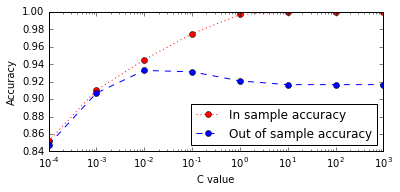
\includegraphics[width=0.7\linewidth]{svm_lin.PNG}
	\caption{SVM performance with a simple linear kernel for various $C$  values(cost).}
	\label{fig:svm_lin}
\end{figure}

\begin{figure}[h!]
	\centering
	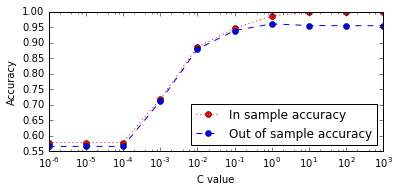
\includegraphics[width=0.7\linewidth]{svm_poly2.PNG}
	\caption{SVM performance with a second-order polynomial kernel for various $C$ values(cost).}
	\label{fig:svm_poly2}
\end{figure}

\begin{figure}[h!]
	\centering
	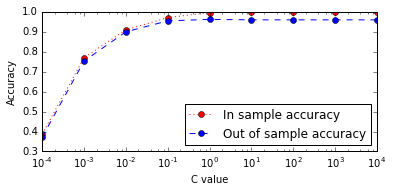
\includegraphics[width=0.7\linewidth]{svm_poly3.PNG}
	\caption{SVM performance with a third-order polynomial kernel for various $C$ values(cost).}
	\label{fig:svm_poly3}
\end{figure}

\begin{figure}[h!]
	\centering
	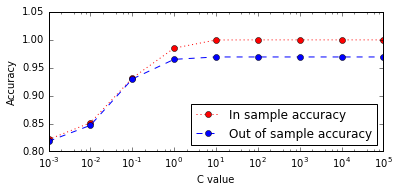
\includegraphics[width=0.7\linewidth]{svm_rbf.PNG}
	\caption{SVM performance with a RBF kernel with $\gamma=0.01$ for various $C$ values(cost).}
	\label{fig:svm_rbf}
\end{figure}

\begin{figure}[h!]
	\centering
	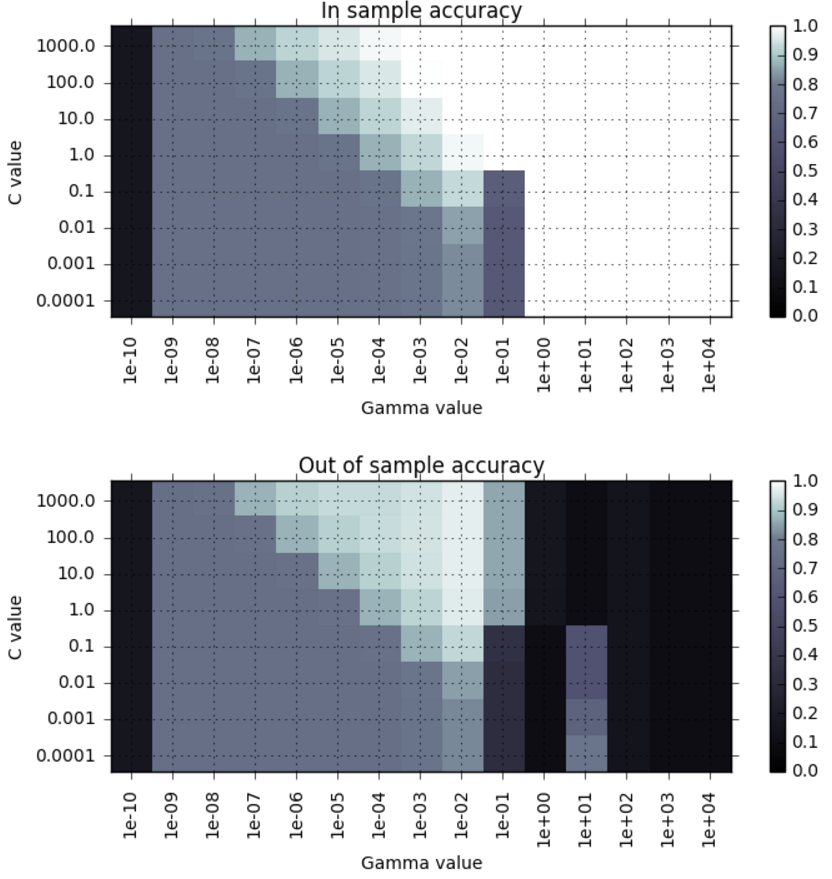
\includegraphics[width=0.9\linewidth]{svm_rbf_grid.PNG}
	\caption{Classification accuracy with a RBF kernel with various $\gamma$- and $C$ values(cost).}
	\label{fig:svm_rbf_grid}
\end{figure}

\begin{table}[h!]
	\centering
	\caption{Classification accuracy of digits with different kernels for the found optimal hyperparameters. }
	\label{tab:svm_accuracy}
	\begin{tabular}{rccc}
		SVM kernel & Validation accuracy & Training accuracy & $C$-value \\ 
		\hline 
		Linear & $93.29\%$ & $94.52\%$ & $0.01$ \\ 
		2th order poly. & $96.16\%$ & $98.74\%$ & $1$ \\ 
		3rd order poly. & $0\%$ & $0\%$ & ?? \\ 
		RBF, $\gamma=0.01$ & $96.94\%$ & $99.98\%$ & $10$ \\ 
	\end{tabular} 
\end{table}

\chapter{Neural Nets with TensorFlow}

\begin{figure}[h!]
	\centering
	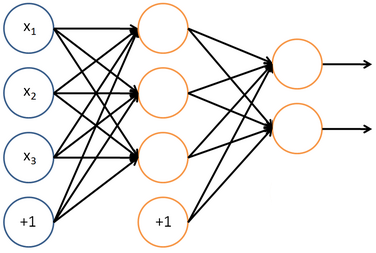
\includegraphics[width=0.4\linewidth]{nn_layout.png}
	\caption{Illustration of a small NN, with one hidden layer. The input vector consists of the $784$ pixel values for an image, the hidden layer has $1024$ nodes, and the output layer has $10$ nodes, one for each digit-class. Biases are added for both computational layers.}
	\label{fig:nn_layout}
\end{figure}

\fixme{Hyperparameters: learning rate, batchsize, epochs to run, }
\fixme{training time}
\fixme{results}

\chapter{Making the best classifier in 2016 ML Class}
\fixme{describe combination of datasets to achieve larger training set}
\fixme{Hyperparameters: learning rate, batchsize, epochs to run, }
\fixme{illustrate convolutional network}
\fixme{results}



	
\end{document}
